\documentclass{article}
\usepackage{graphicx} % Required for inserting images

\title{Trabajo Práctico 2 - Teoría de Juegos}
\author{Juani Elosegui}
\date{Septiembre 2024}

\begin{document}
    \maketitle

    \newpage
    
    \section*{Problema 1.}
        \subsection*{Respuesta}
            Sabemos que cuando una estrategia mixta es parte de un Equilibrio de Nash, el jugador no va a tener incentivos para desviarse de esa estrategia mixta.\\
            \\
            Estar en un Equilibrio de Nash en estrategias mixtas implica que el pago de esa estrategia mixta será igual al pago esperado de cada una de las estrategias puras que forman parte de las mixtas.
            
            Si tengo dos estrategias puras -llámense estrategias A y B- y elijo una estrategia mixta que le asigna probabilidades P(A) = $p$ y P(B) = $1-p$, si esta estrategia mixta está en equilibrio, el pago esperado de jugar A debe ser igual al pago esperado de jugar B.\\
            \\
            Además, estar en un Equilibrio de Nash también implica que un jugador debe ser indiferente entre las estrategias puras que forman a la estrategia mixta, porque si una estrategia pura tuviera un pago esperado mayor que la otra, un jugador siempre eligiría la estrategia que pague más.

            Esto es, si sé que la estrategia A me podría pagar más que la estrategia B, no hay discusión: claramente jugaría A. Si elijo una sola estrategia pura, ya no estaríamos hablando de estrategias mixtas, porque P(A) = $1$.

    \newpage

    \section*{Problema 2.}
        \subsubsection*{Respuesta inciso a)}
            No existe un equilibrio en estrategias puras en el que ambos jugadores eligen $H$, ya que ambos preferirían cambiar a $D$ para evitar el costo de la pelea.
            \\
            Tampoco es un equilibrio que ambos jugadores elijan $D$, ya que cualquiera de ellos tendría el incentivo de cambiar a $D$ para obtener todo el recurso.
            \\
            Concluyendo, no hay equilibrios de Nash en estrategias puras en este juego.
            \\
            \\
            Por otro lado, si quisiera encontrar un equilibrio en estrategias mixtas. $J1$ será indiferente entre jugar $H$ ó $D$ si el pago esperado de ambas estrategias es el mismo. Lo mismo ocurre para $J2$.
            \\
            Para $J1$, el pago esperado de jugar $H$ es:
            \[p \cdot \frac{V - C}{2} + (1 - p) \cdot V\]
            Y el pago esperado de jugar $D$ es:
            \[p \cdot 0 + (1 - p) \cdot \frac{V}{2}\]
            Si igualamos los pagos esperados y despejamos $p$, obtenemos que   
            \[p = \frac{V}{C}\]
            \\
            Por lo tanto, el equilibrio de Nash en mixtas será cuando ambos jugadores jueguen $H$ con probabilidad $p = \frac{V}{C}$ y $D$ con probabilidad $1-p = \frac{C - V}{C}$. Como el juego es simétrico, sabemos que $p = q$.

        \subsubsection*{Respuesta inciso b)}
            El equilibrio en estrategias mixtas nos dice que $J1$ y $J2$ jugarán $H$ con probabilidad $p = q = \frac{V}{C}$, y $D$ con probabilidad $1 - p = 1 - q = \frac{C - V}{C}$.
            \\
            Si aumenta $V$, la probabilidad de que los jugadores jueguen $H$ aumenta, porque $p = \frac{V}{C}$ aumentará si $V$ lo hace.
            \\
            Análogamente, si aumenta $C$, la probabilidad de que los jugadores jueguen $H$ disminuye, porque $p = \frac{V}{C}$ disminuye si $C$ lo hace.
    \newpage
        
    \section*{Problema 3.}
        \subsubsection*{Respuesta inciso a)}
            El pago esperado de la estrategia mixta de \{P(T) = 0, P(M) = $0.5$, P(B) = $0.5$\} es el siguente cuando $J2$ juega $L$:        
            \[0 \cdot 1 + \frac{1}{2} \cdot 4 + \frac{1}{2} \cdot 0 = 2\]
            \\
            El pago esperado de la estrategia mixta cuando $J2$ juega $R$:
            \[0 \cdot 1 + \frac{1}{2} \cdot 0 + \frac{1}{2} \cdot 3 = 1,5\]
            \\
            Si calculamos el pago esperado de la estrategia pura $T$ si $J2$ juega $L$:
            \[ 1 \cdot 1 = 1\]
            \\
            Si $J2$ juega $R$, es lo mismo:
            \[1 \cdot 1 = 1\]
            \\
            Como la estrategia mixta tiene pagos esperados mayores que los posibles de $T$, se puede concluir que esta estrategia mixta domina estrictamente a $T$.

        \subsubsection*{Respuesta inciso b)}
            Necesitamos encontrar combinaciones de estrategias puras (que luego compondrán a una estrategia mixta) tales que dominen a $T$, es decir, que paguen más de $1$. Las estrategias puras pasan ahora a llamarse $p, q, r$ como nombre genérico, abstrayéndonos de $T, M, B$.
            \\
            El valor esperado de $(p, q, r)$ cuando $J2$ juega $L$ es:
            \[ p \cdot 1 + q \cdot 4 + r \cdot 0 = \]
            \[p+4q\]
            \\
            El valor esperado de $(p, q, r)$ cuando $J2$ juega $R$ es:
            \[p \cdot 1 + q \cdot 0 + r \cdot 3 =\]
            \[p+3r\]
            \\
            Para que una estrategia mixta domine estrictamente a $T$, se necesita que se cumpla esto:
            \[p + 4q > 1\]
            \[\wedge\]
            \[p+3r > 1\]
            \\
            Si tenemos que $(\frac{1}{2},\frac{1}{2},0)$:
            \[p+4q = \frac{1}{2}+4\cdot\frac{1}{2} = 2.5 > 1\]
            Esto cumple la condición. Pero,
            \[p+3r = \frac{1}{2}+0 = 0.5 < 1\]
            No la satisface.
            \\
            Si tenemos que $(0, \frac{1}{2}, \frac{1}{2})$, sí la satisface:
            \[p+4q = 0+2 = 2 > 1\]
            \[\wedge\]
            \[p+3r = 0 + 1.5 = 1.5 > 1\]
            Por lo tanto, $(0, \frac{1}{2}, \frac{1}{2})$ es una de las posibles estrategias que dominan estrictamente a $T$.

            \newpage
            
    \section*{Problema 4.}
        \subsubsection*{Respuesta inciso a)}
            \begin{figure}[h]
                \centering
                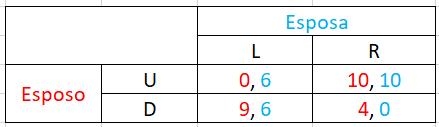
\includegraphics[width=0.5\linewidth]{fig7.png}
            \end{figure}
                
        \subsubsection*{Respuesta inciso b)}
            Los equilibrios son $\{(D, L),(U,R)\}$

        \subsubsection*{Respuesta inciso c)}
            Supongamos que $p$ ahora es la probabilidad de que el esposo elija $U$, y $1-p$ la probabilidad de que elija $D$.
            \\
            Supongamos también que $q$ es la probabilidad de que la esposa elija $L$, y $1-q$ la probabilidad de que elija $R$.

            Igualando los pagos esperados de $U, D$ del esposo, obtenemos que:
            \[0 \cdot q + 10(1-q) = 9 \cdot q + 4 \cdot (1-q)\]
            \[10 - 10q = 5q+4\]
            \[6 = 15q\]
            \[q = \frac{6}{15}\]
            \[q = 0.4\]
            \\
            Igualando los pagos esperados de $L, R$ de la esposa, obtenemos que:
            \[6 \cdot p + 6 \cdot (1-p) = 10 \cdot p + 0 \cdot (1-p)\]
            \[6 = 10p\]
            \[p = \frac{6}{10}\]
            \[p = \frac{3}{5}\]
            \[p = 0.6\]
            \\
            Concluyendo, vemos que el equilibrio en estrategias mixtas sucede cuando $p = 0.6$ y $q = 0.4$.

        \newpage

        \subsubsection*{Respuesta inciso d)}
            \begin{figure}[h]
                \centering
                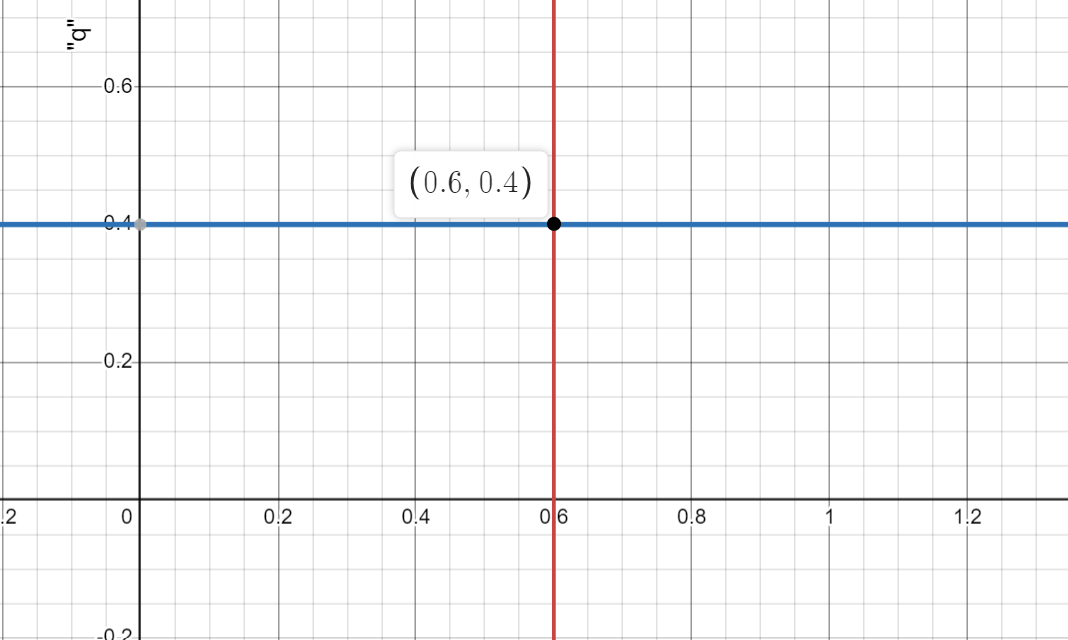
\includegraphics[width=0.75\linewidth]{fig8.png}
            \end{figure}

            El punto gris representa el equilibrio de Nash: $(p=0.6, q=0.4)$.
\end{document}
